\section{Clique}

A clique in an undirected graph $G=(V,E)$ is sa set $S \subseteq V$ such that for all pairs of distinct $u, v \in S$, $\{u,v\} \in E$.

$$
\Clique = \{ \encoding{G,k} \mid \text{$G$ is a graph, $k \in \N$ and $G$ has a clique of size $k$ }\}
$$

\begin{theorem}
    CLIQUE is NP-compelte.
\end{theorem}

\begin{proof}
    Clearly, CLIQUQE $\in \NP$. To show that CLIQUE is NP-hard, we will show the reduction $\threeSAT \leq_p \Clique$.

    Given a 3CNF formula $\phi$, construct in polynomial time $\encoding{G_{\phi},k_{\phi}}$ such that
    $$
    \text{$\phi$ is satisfiable} \iff \text{$G_{\phi}$ has a clique of size $k$}
    $$
    Suppose $\phi = (a_1 \lor b_1 \lor c_1) \land (a_2 \lor b_2 \lor c_2) \lor \cdots \lor (a_k \lor b_k \lor c_k)$ with $k$ clauses and 3 literals per clause.

    We construct $G$ such that it has $k$ groups of 3 vertices (giving us $3k$ vertices) where each vertex is labeled according to a literal in a clause. We connect all pairs of vertices except:
    \begin{itemize}
        \item vertices in the same triple (same clause)
        \item vertices with contradictory labels ($x_i$ and $\overline{x_i}$)
    \end{itemize}
    Now assume that $\phi$ is satisfiable, then there exists some assignment of variables that satisfies $\phi$. Take such satisfying assignment. In this assignment, there must be at least one true literal in each clause. In each triple, pick any one vertex corresponding to the true literal. These vertices form a $k$-clique containing $k$ vertices, distinct triples (because there is no edge among vertices within the same triple), and no contradicting labels (becuase there is no edge between contradictory labels).

    Suppose a graph $G$ has a $k$-clique. Then, no two vertices in the clique are in the same triple. Each triple has exactly one vertex in the clique. Assign values to variables so that all clique nodes are true literals (this is possible since there is no contradictory labels in clique). This assignment satisfies $\phi$. Therefore, $\phi$ is satisfiable.
\end{proof}

Now consider the language $k$-CLIQUE. In this language, $k$ is fixed.
$$
\text{$k$-CLIQUE} = \{ \encoding{G} \mid \text{$G$ is an undirected graph with a clique of size $k$ }\}
$$
\begin{theorem}
    $k$-CLIQUE $\in \p$ for all $k$.
\end{theorem}

\begin{proof}
    Check all ${n \choose k}$ subset of vertices. Since $k$ is fixed, this number of subset needs be checked is polynomial in $n$.
\end{proof}

\section{Independent Sets}

$G=(V,E)$, $S \subseteq V$ is an independent set in $G$ if $\encoding{u,v}\not\in E$ for all distinct $u,v \in S$.

$$
\text{IND-SET} = \{\encoding{G,k} \mid \text{$G$ is a graph which contains an independent set of size $k$}\}
$$

\begin{theorem}
    IND-SET is NP-complete.
\end{theorem}

\begin{proof}
    We show that CLIQUE $\leq_p$ IND-SET.
\end{proof}

\section{Vertex Cover}

Let $G=(V,E)$ be an undirected graph. $S \subseteq V$ is a vertex cover for $G$ if every edge in $G$ has at least one endpoint in $S$.

$$
\text{VERTEX-COVER} = \{ \encoding{G,k} \mid \text{$G$ has vertex color of size $k$}\}
$$

\begin{theorem}
    VERTEX-COVER is NP-complete.
\end{theorem}

\begin{proof}
    Showing VERTEX-COVER $\in \NP$ is easy. We show VERTEX-COVER is NP-hard by showing
    $$
    \text{IND-SET} \leq_p \text{VERTEX-COVER}
    $$
    For the reduction, we map $\encoding{G,k}$ to $\encoding{G,|V|-k}$. We claim that $G=(V,E)$ where $S \subseteq V$ is an independent set in $G$ if and only if $V-S$ is a vertex cover.
\end{proof}

\section{Coloring}

An undirected graph $G$ is $k$-colorable if there is a map $f:\, V \to \{1,2\ldots,k\}$ such that for every edge $(u,v) \in E$, $f(u) \neq f(v)$.

\begin{theorem}
    2COL $\in \p$.
\end{theorem}

\begin{proof}
    Run BFS. Greedily assign colors by alternating coloring for each level.
\end{proof}

\begin{theorem}
    3COL is NP-complete.
\end{theorem}

\begin{proof}
    We show that 3SAT $\leq_p$ 3COL.

    \begin{figure}[htbp]
        \centering
        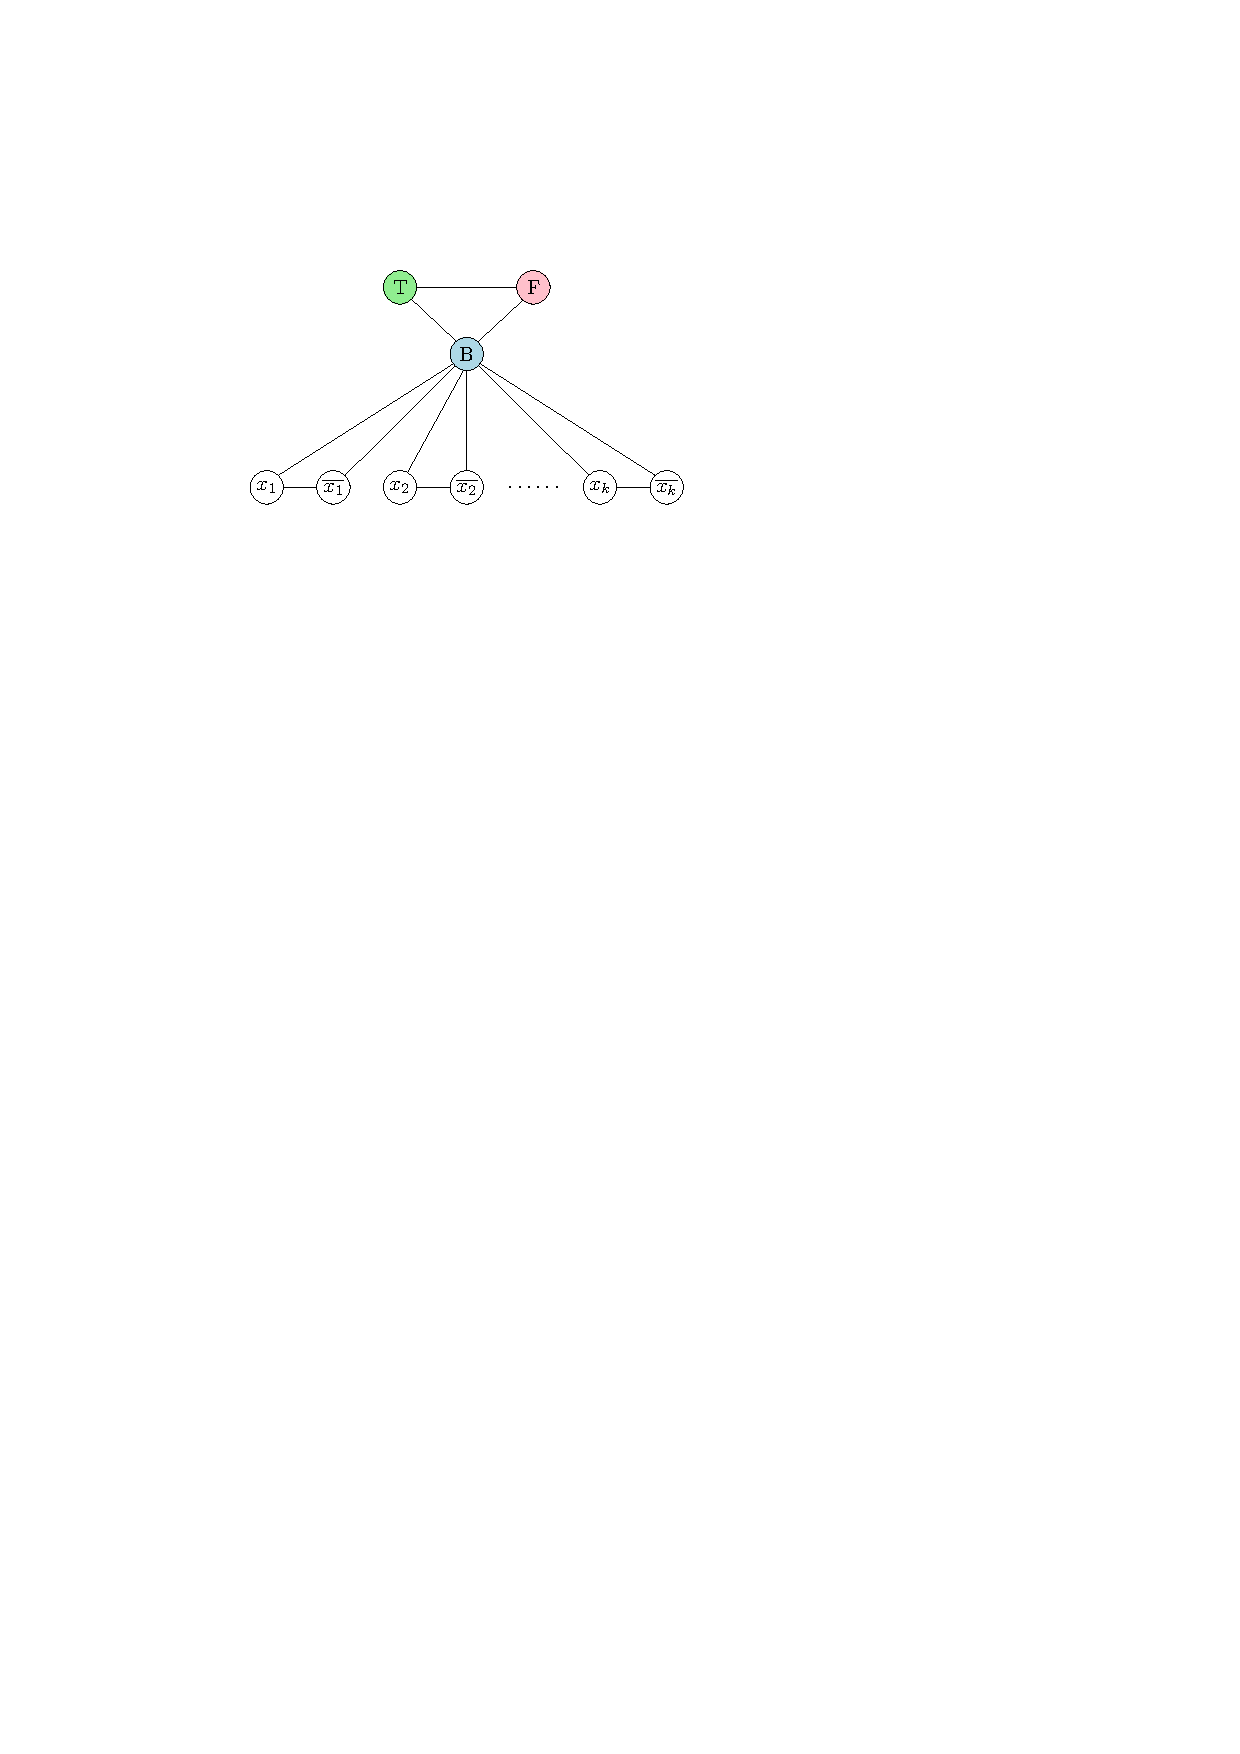
\includegraphics[width=0.4\linewidth]{3color-palette-variable-construction.pdf}
        \caption{Construction that ensures that a coloring corresponds to a valid truth assignment.}
        \label{fig:3color-valid-construction}
    \end{figure}

    \begin{figure}[htbp]
        \centering
        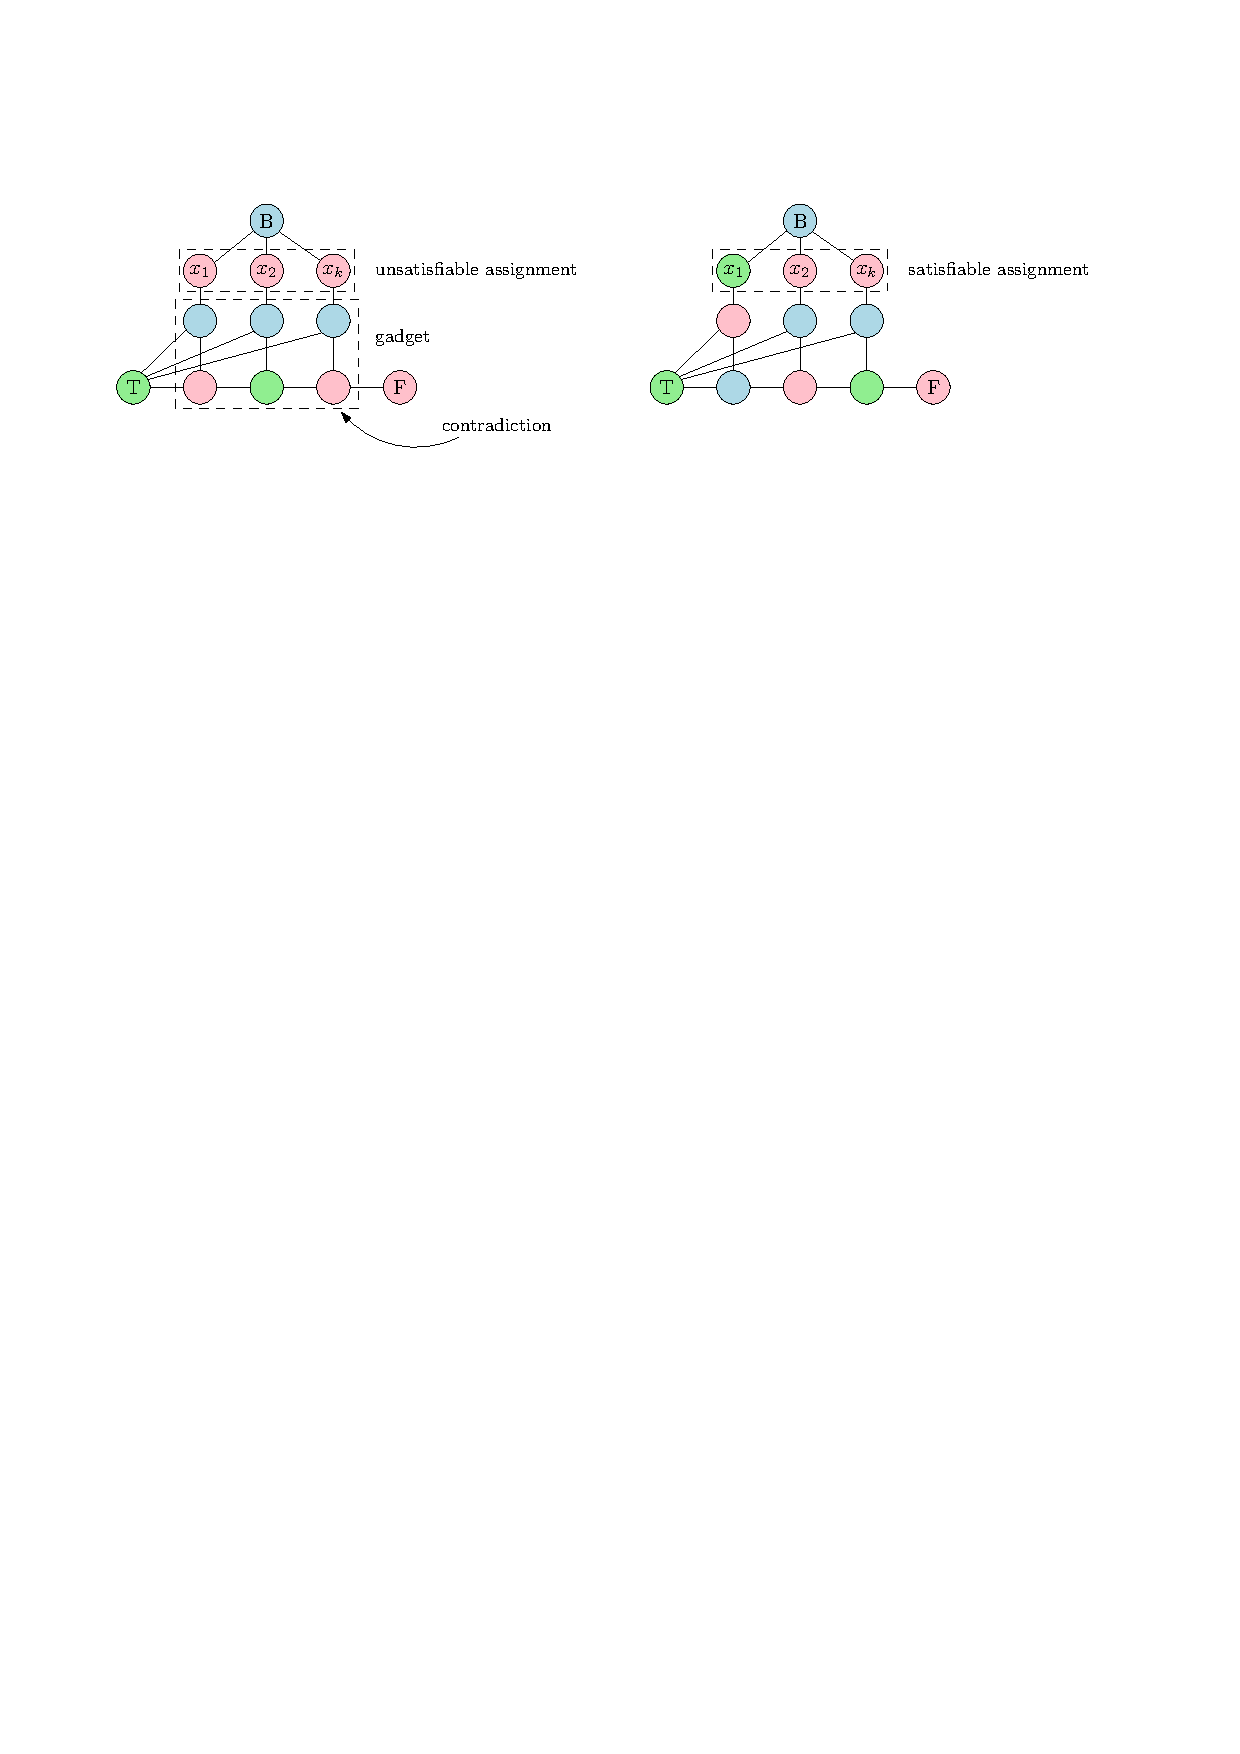
\includegraphics[width=0.8\linewidth]{3color-gadget-construction.pdf}
        \caption{Construction using gadgets that ensures only satisfiable truth assignment can be colored.}
        \label{fig:3color-gadgets-construction}
    \end{figure}

    An alternative construction uses the OR-gadget. The OR-gadget forces the three vertices within the gadget to have different colors. This, in turn, forces a contradiction at the output gadget when we have all literals being false.

    \begin{figure}[htbp]
        \centering
        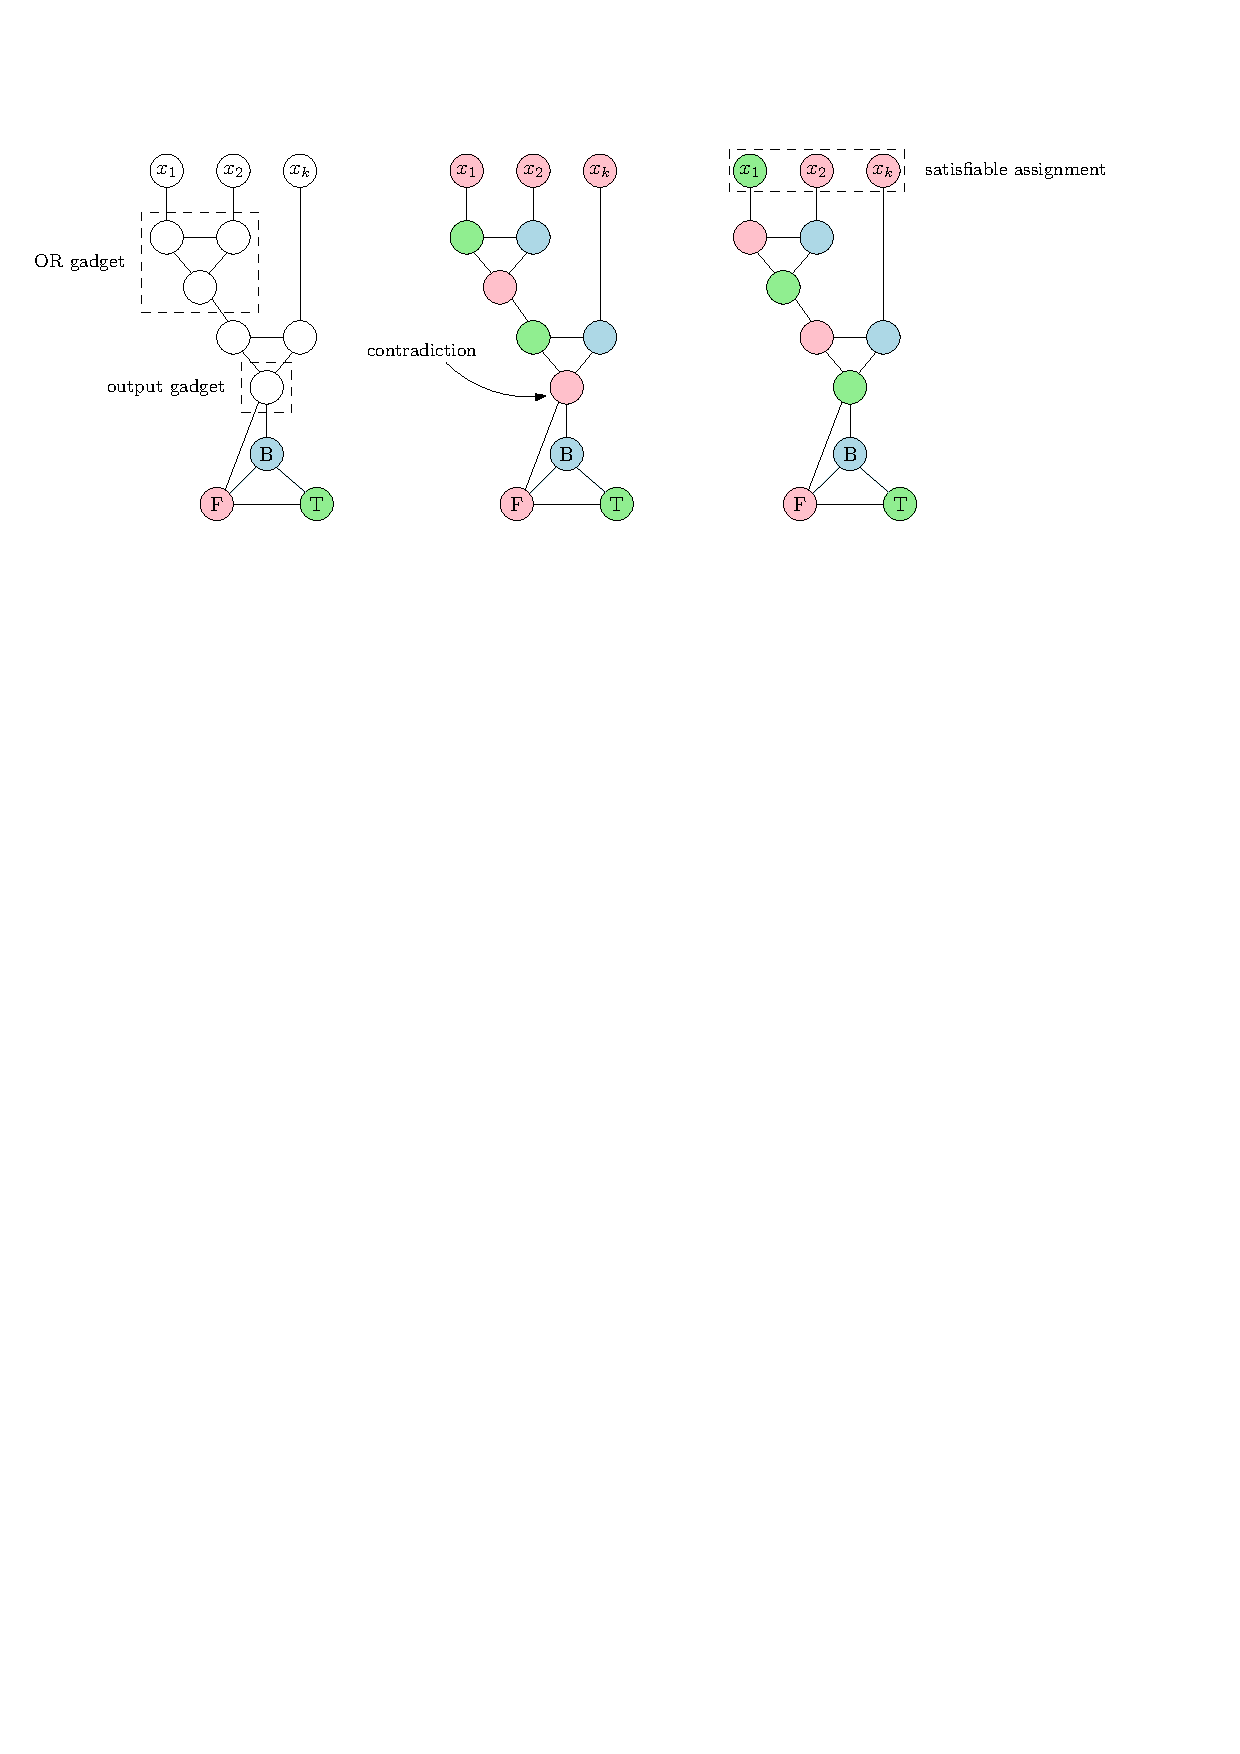
\includegraphics[width=0.9\linewidth]{3color-gadget-alternative-construction.pdf}
        \caption{Construction using gadgets that ensures only satisfiable truth assignment can be colored.}
        \label{fig:3color-gadgets-alternative-construction}
    \end{figure}
\end{proof}

\section{Subset Sum}

Given a collection of numbers $x_1,\ldots,x_k$ and a target $t$, is there a subcollection adding up to $t$.
$$
\text{SUBSET-SUM} = \{\encoding{s,t} \mid \text{$s = \{x_1,\ldots,x_k\}$ and for some $\{y_1,\ldots,y_i\} \subseteq \{x_1,\ldots,x_k\}$, $\Sigma y_i = t$}\}
$$

\begin{proof}
    
\end{proof}